\title{A pilot study examining the diet of introduced Alaska blackfish (\textit{Dallia pectoralis} T.\ H.\ Bean, 1880) in Kenai, Alaska, by metabarcoding}

\subtitle{\doi{10.----------}}

\author{by Matt Bowser\footnote{US Fish \& Wildlife Service, Kenai National Wildlife Refuge, Soldotna, Alaska, \email{matt\_bowser@fws.gov}}and Apphia Bowser}

\maketitle

\end{multicols}
\begin{figure}[H]
\begin{center}
%\vspace{2mm}
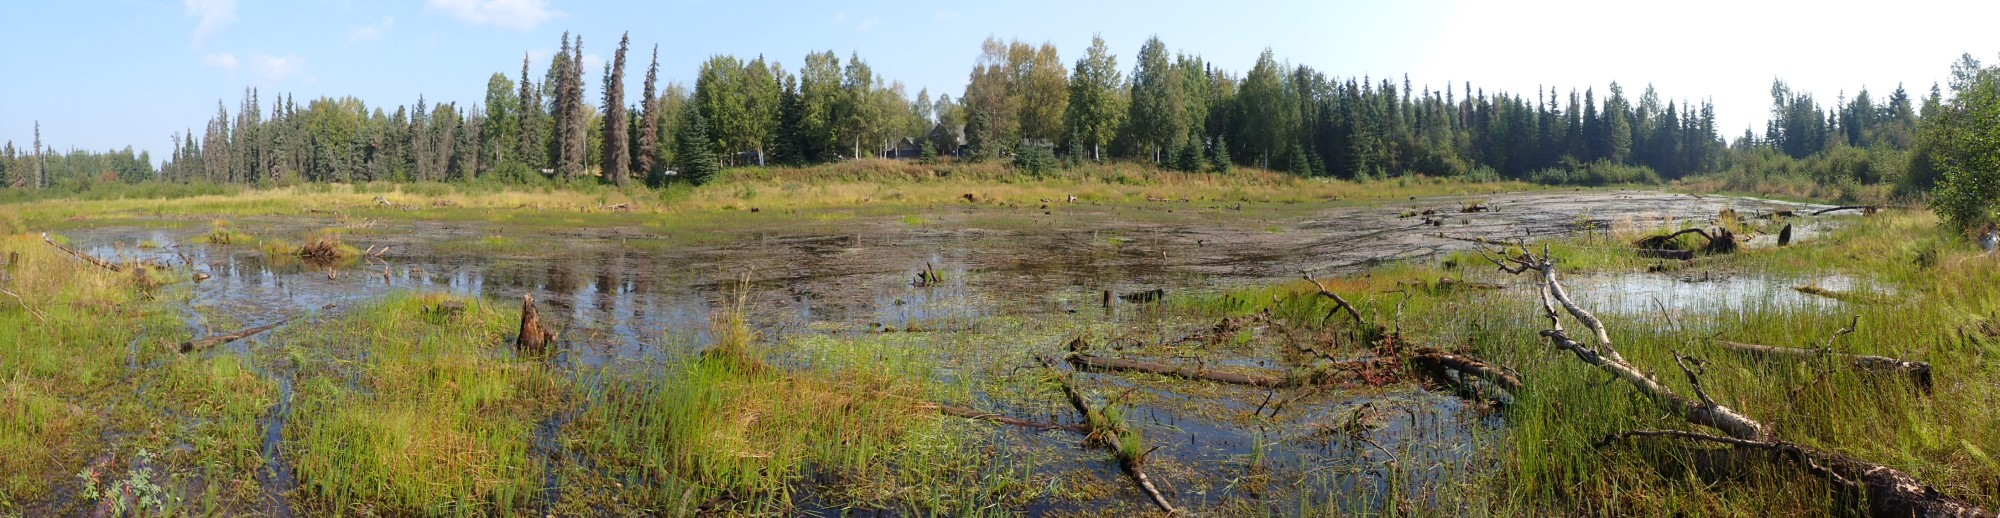
\includegraphics[width=\textwidth]{img/blackfish_pond.jpg}
\caption{Panoramic montage of a pond off of the Kenai Spur Highway and Candlelight Drive, the locality from which blackfish specimens were collected. A full resolution image is available on Arctos (\doi{10.7299/X7ZP46FP}).}
\label{blackfish_pond}
\end{center}
\end{figure} 
\begin{multicols}{2}   

\section{Introduction}

Last year we  wrote about some food items of the Alaska blackfish, \textit{Dallia pectoralis} T.\ H.\ Bean, 1880 \citep{Bowseretal2019},  a fish species that is native to part of Alaska, but not the Kenai Peninsula \citep{Eidametal2016, Bowser2018}. We wanted to learn more about how these introduced fish may alter the ecology of Kenai Peninsula waters, especially how blackfish may affect native fish species through competition for invertebrate prey.

\section{Methods}

We collected blackfish under Alaska Department of Fish \& Game permit Number SF2019-111.

On 23 August 2019 we collected blackfish from a small, shallow pond in Kenai, Alaska (60.5681~\textdegree{}N, -151.1901~\textdegree{}W $\pm$ 40~m) \citep{bowser2019}, the same pond from which we had obtained blackfish the previous year \citep{Bowseretal2019}. This pond (Figure \ref{blackfish_pond}) is fed by a small inlet stream and its level is maintained by a dam at the outlet, from which the stream flows through the Kenai Golf Course and into the Kenai River. There is little open water; most of the pond is thickly filled with \textit{Potamogeton} and flocculent iron bacterial scum. Only one other fish species, a single specimen of a nine-spined stickleback (\textit{Pungitius pungitius} (Linnaeus, 1758),  
\url{https://www.inaturalist.org/observations/31561030}), was observed in this pond.

We attempted to collect blackfish from other reaches of the stream below this pond where there would have been more potential for interaction between blackfish and other fish species, but found only small, juvenile blackfish downstream. 

The collected blackfish were placed on ice in a cooler, transported to the lab, and frozen. Later we thawed five adult blackfish, measured their lengths, dissected out their entire guts, and squeezed gut contents into vials of UniGard -100 propylene glycol antifreeze.

Vials of gut contents were shipped to \acr{RTL} Genomics in Lubbock, Texas (\url{https://rtlgenomics.com/}) for RTL Genomics' standard microbial diversity assay using the \textit{mlCOIint}/\textit{jgHCO2198} (GGWACWGGWTGAACWGTWTAYCCYCC/TAIACYTCIGGRTGICCRAARAAYCA) primer set.

Extraction methods, sequencing methods, and resulting raw sequence data are provided in \citet{BowserBowser2020}.

\end{multicols}
\begin{figure}[H]
\begin{center}
%\vspace{2mm}
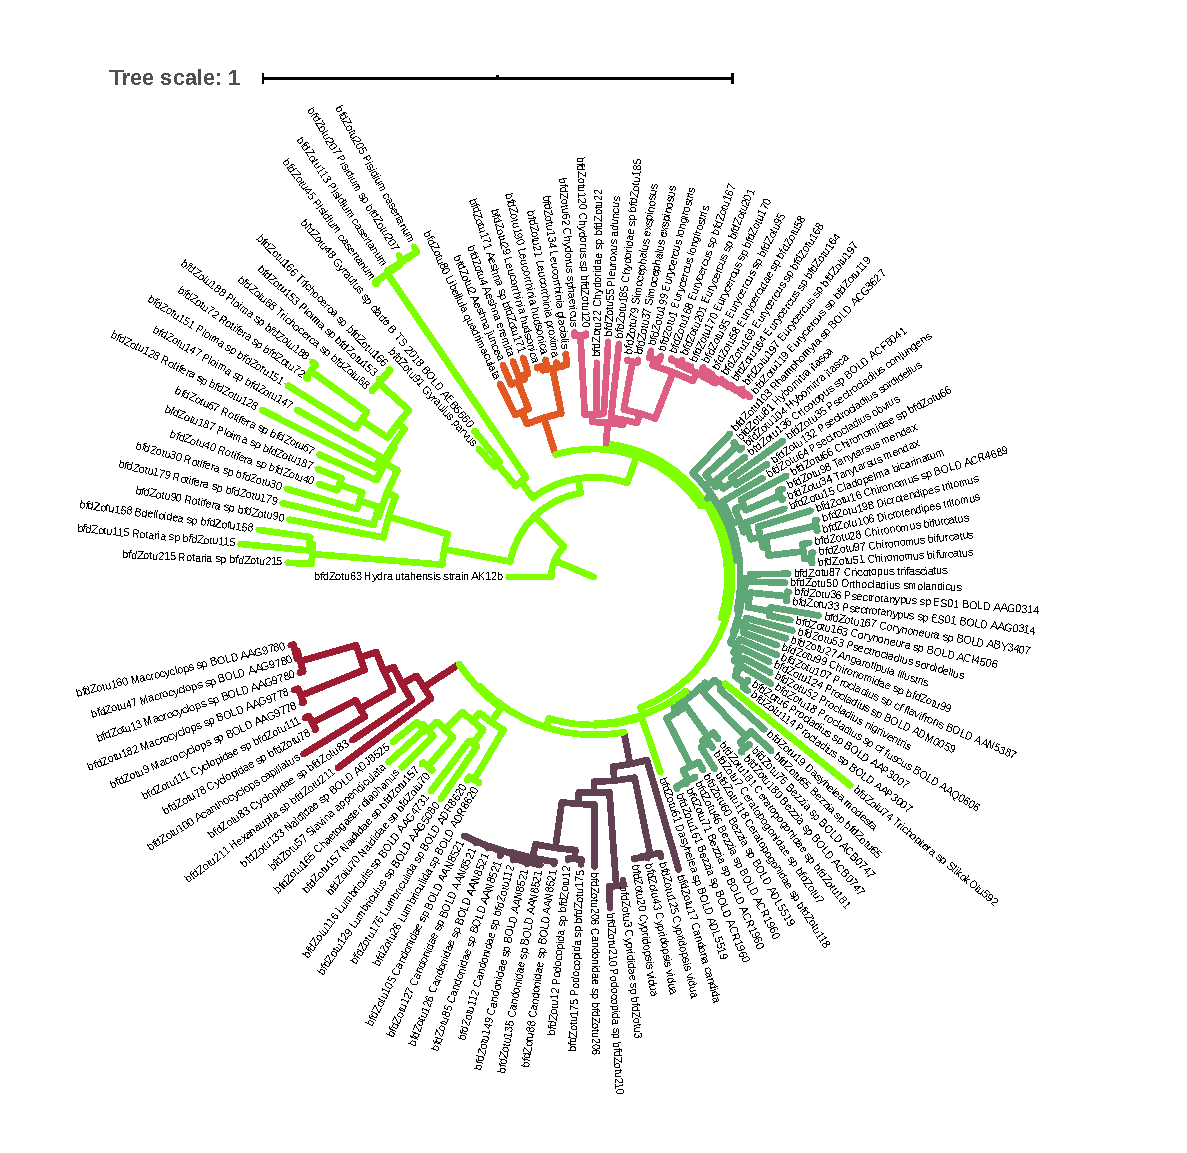
\includegraphics[width=\textwidth]{img/blackfish_phylo.pdf}
\caption{Phylogram of retained \acr{ESV} sequences. Colors representing major groups are the same as in Figure \ref{blackfish_pie_chart}. The tree can be viewed interactively or downloaded from \url{https://itol.embl.de/tree/16415961276811585237767}.}
\label{blackfish_phylo}
\end{center}
\end{figure} 
\begin{multicols}{2} 

Raw reads were processed using the \acr{SCVUC} \acr{COI} metabarcode pipeline version 4.3.0 (\url{https://github.com/Hajibabaei-Lab/SCVUC_COI_metabarcode_pipeline}). This pipline runs SeqPrep \citep{StJohn2016}, \acr{CUTADAPT} \citep{Martin2011}, \acr{VSEARCH} \citep{Rognes2016}, \acr{UNOISE} \citep{Edgar2016}, and the RDP classifier \citep{Wang2007} using the \acr{COI} Classifier v4 reference dataset \citep{PorterHajibabaei2018}. Processing steps were run via Snakemake \citep{KosterRahmann2012}. Our \acr{SCVUC} configuration file \citep{Bowser2020config} and snakefile \citep{Bowser2020snakefile} are available on Arctos.

The resulting exact sequence variants (\acr{ESV}s) were also compared to \acr{ESV}s obtained by \citet{Bowseretal2020} \citep[dataset: ][]{, Bowseretal2020sup5}, sequences from the Alaska terrestrial arthropod \acr{DNA} barcode \acr{COI} reference library (\url{https://github.com/mlbowser/AKTerrInvCOILib}), and a \acr{FASTA} file of sequences from the authors' LifeScanner (\url{http://lifescanner.net/}) records (\url{http://www.boldsystems.org/index.php/Public_SearchTerms?query=DS-BOWSER}) using \verb|vsearch --usearch_global|. We also submitted our \acr{ESV}s to \acr{NCBI} \acr{BLAST} \citep{Johnsonetal2008} and \acr{BOLD} \acr{ID} Engine \citep{Ratnasinghametal2007} searches  and scrutinized the results. We followed the guidlines of \citet{Sigovinietal2016} when assigning provisional names.

We removed all reads identified as \textit{Dallia pectoralis}; \textit{Bos taurus} Linnaeus, 1758; and all non-animals. The small numbers of \textit{Bos taurus} reads likely came from bovine serum albumin added during \acr{DNA} amplification. As a final check of identifications, we generated a phylogeny of the filtered \acr{ESV}s using NGPhylogeny.fr, ``NGPhylogeny Analyse - FastME/OneClick'' option \citep{DesperGascuel2002, CriscuoloGribaldo2010, JunierZdobnov2010, KatohStandley2013, Lefortetal2015, Lemoineetal2019} and examined the tree using i\acr{TOL} \citep{LetunicBork2019} (Figure \ref{blackfish_phylo}). The \acr{FASTA} file of retained \acr{ESV} sequences is available from Arctos \citep{Bowser2020bfdfas}. 


To prevent reporting false postive occurrences, we removed occurrences represented by $\leq 0.05\%$ of the total number of reads of an \acr{ESV}. Complete analysis details are provided in \citet{bowser2020}.

We tried to follow the guidelines of \citet{Penevetal2017} by publishing occurrence data on Arctos, which supplies occurrence data to \acr{GBIF}. Specimen records, images, and other related files have been made available via an Arctos project at \url{http://arctos.database.museum/project/10003367}.

\section{Results}

The retained 131 Exact Sequence Variants (Figure \ref{blackfish_phylo} ) were represented by 63,172 reads. The \acr{ESV}s were assigned to 103 uniquely identified food items. Arthropods represented by 62,166 (98\%) of the reads, followed by rotifers (431 reads, 0.7\%), annelid worms (384 reads, 0.6\%), molluscs (160 reads, 0.3\%), and one species of hydra (\textit{Hydra utahensis} Hyman, 1931, strain AK12b \textit{sensu} \citet{Martinezetal2010}, 31 reads, 0.05\%). The most abundant groups in terms of read abundances were dragonflies (32\%), flies (24\%), cladocerans (20\%), ostracods (16\%), and copepods (7\%) (Figure \ref{blackfish_pie_chart}).

\begin{figure}[H]
\begin{center}
\vspace{2mm}
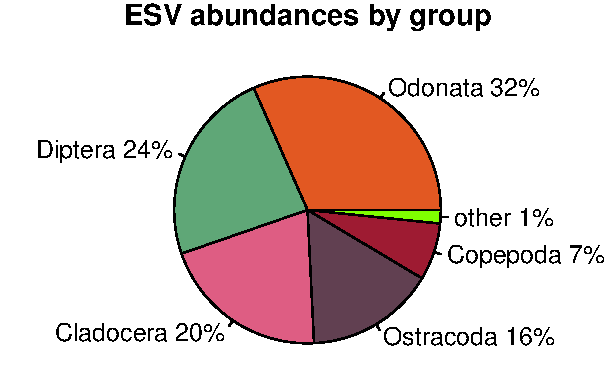
\includegraphics[width=8cm]{img/blackfish_pie_chart.pdf}
\caption{Percentages of \acr{ESV} abundances in blackfish diet by taxonomic group.}
\label{blackfish_pie_chart}
\end{center}
\end{figure} 

Of the 103 unique identifications, 13 were comparatively abundunt, each representing $\geq 1$\% of the total number of reads (Figure \ref{blackfish_diet_items}). All of the reads of \textit{Aeshna eremita} Scudder, 1866 (Odonata: Aeshnidae), the most abundant species identified, came from a single blackfish. We detected \textit{Aeshna juncea} Linnaeus, 1758, the second most abundant species in our samples, from three fish. Ceratopogonidae sp.\ bfdZotu7 was both abundant and frequent in our samples, detected in gut contents of four out of five blackfish.

The relative abundance of each food item in terms of read abundances varied widely among the five blackfish individuals. For each fish, a different prey species was the most abundant food item.

Three of the most abundant \acr{ESV}s could be associated with niether described species nor \acr{BOLD} Barcode Index Numbers \citep{Ratnasinghametal2013}.  The \acr{ESV} identified as Ceratopogonidae sp.\ bfdZotu7 was 98.71\% similar ($p$-dist) to a private record on \acr{BOLD}. The \acr{ESV} tentatively identified as Cyprididae sp.\ bfZotu3 had no close matches in \acr{BOLD} or \acr{BAST}n search results, but the closest matches (83.99\% similarity) were Cyprididae. The \acr{ESV} identified as Podocopida sp.\ bfdZotu12 was closest (95.44\% similar) to a sequence from an ostracod specimen identified as Podocopida (\acr{BOLD} processid: \BOLD{OZFWC245-11}).

\end{multicols}
\begin{figure}[H]
\begin{center}
%\vspace{2mm}
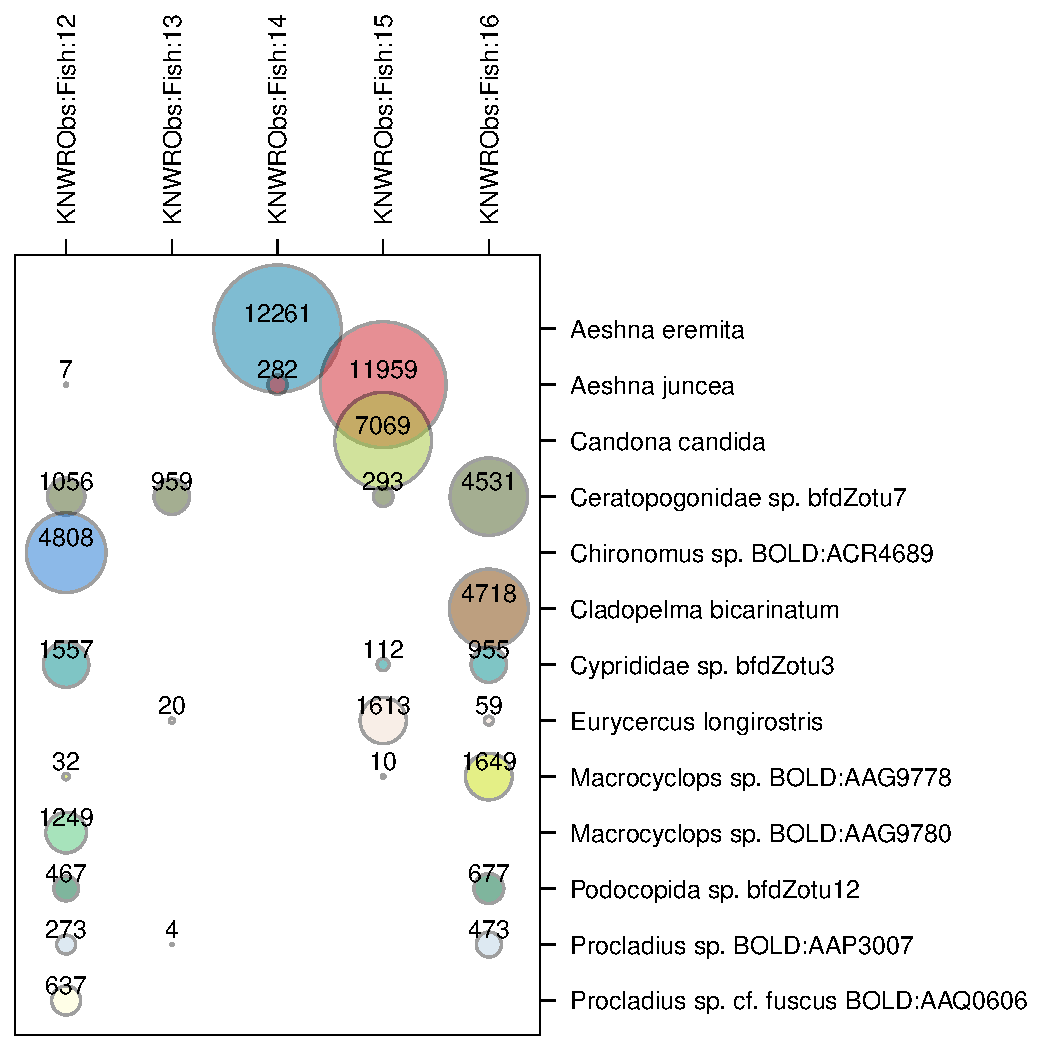
\includegraphics[width=13cm]{img/blackfish_diet_items.pdf}
\caption{Read abundances of identified food items from each of five blackfish specimens. Only food items that represented $\geq 1$\% of the total number of reads were included. The area of each circle is proportional to read abundances.}
\label{blackfish_diet_items}
\end{center}
\end{figure} 
\begin{multicols}{2} 

Some of the \acr{ESV}s matched \acr{DNA} barcode sequences from locally collected entities that had not been associated with a formally described species. These included Lumbriculida sp.\ BOLD:ADR8620, a lumbriculid worm collected previously from near Nordic Lake, Soldotna (\acr{BOLD} processid: \BOLD{MOBIL6661-18}); \textit{Lumbriculus} sp.\ BOLD:AAG4731, another lumbriculid worm documented from a temporary pool in Soldotna (\acr{BOLD} processid: \BOLD{MOBIL1270-16}); and Trichoptera sp.\ SlikokOtu592, an \acr{ESV} from near Headquarters Lake documented by \citet{Bowseretal2020} (Arctos \acr{GUID}: \guid{UAMObs:Ento:239239}).

Seven chironomid species identified from our samples appeared to be new distribution records for Alaska. These were 
\textit{Chaetocladius conjugens} Brundin, 1947; 
\textit{Chironomus bifurcatus} Wuelker, Martin, Kiknadze, Sublette \& Michiels, 2009; 
\textit{Cladopelma bicarinata} (Brundin, 1947);
\textit{Cricotopus trifasciatus} (Meigen, 1813);
\textit{Dicrotendipes tritomus} (Thienemann \& Kieffer, 1916);
\textit{Orthocladius smolandicus} Brundin, 1947; and
\textit{Procladius nigriventris} (Kieffer, 1924).

\section{Discussion}

It appeared that the adult blackfish that we collected had recently consumed exclusively invertebrates, mostly arthropods. No \acr{DNA} from other fish species was detected. It should be noted, however, that other fish were comparatively rare in this pond. A single nine-spined stickleback was the only other fish documented. It may have been possible that juvenile blackfish were consumed by adult blackfish. These would not have been detected because all blackfish reads were removed from the analysis.

Overall, our results are consistent with other studies of blackfish diet \citep{OstdiekNardone1959, Chlupach1975, Gudkov1998, Eidam2015, Eidametal2016, Bowseretal2019} which collectively show that the most important prey groups
include cladocerans, ostracods, flies, dragonflies, snails, caddisflies,
and copepods. What separates our results from previous studies is that metabarcoding methods yielded much finer identifications, allowing us to document which species were consumed by blackfish. In previous studies, almost all identifications were coarse, with identifications lumped by orders or even higher-level groupings.

The variation in abundances of food items across the five blackfish individuals suggests that these fish are opportunistic, consuming whatever invertebrates they find and not seeking out any particular kind of prey item. It was surprising that we found none of the food items documented by \citet{Bowseretal2019} from blackfish from the same pond. Some differences in diet might have been expected due to season variation. \citet{Bowseretal2019} had collected blackfish on 18--19 October, two months later than our 23 August collecting date. Some of the food items documented by \citet{Bowseretal2019} were terrestrial wetland inhabitants that had likely become available to the blackfish due to flooding at the time. The water level of the pond was much lower when we sampled in August 2019 due to a warm, dry summer. Even with these differences in sampling date and water levels, we had expected to document at least some of the same species. The observed lack of overlap of observed prey items between the two studies supports our conclusion that blackfish are highly opportunistic.   

%Some of the most abundant food items were common species with widespread distributions. \textit{Candona candida} (O.F.Müller, 1776) is an ostracod with a worldwide distribution \citep{Delorme1970} that is found in a wide variety of freshwater habitat types \citep{Alkalajetal2019}. The cladoceran \textit{Eurycercus longirostris} Hann, 1982 is widespread in North America \citep{Bekkeretal2012}.

The rotifer \acr{ESV}s and other small-bodied invertebrates we observed may have been prey items of the blackfish or they may have been eaten by arthropods that were then eaten by blackfish. 

It should be noted that, due to potential biases related to metabarcoding methods, the relative read abundances that we report may not be directly related to the relative proportions of food items in the diets of the blackfish that we collected \citep[see][for an overview]{Deagleetal2018}. Regardless of potential metabarcoding biases due to differences in recovery and amplification of target \acr{DNA} across taxonomic groups, we believe that some of the differences in the wide range of read abundances that we observed had to do with how recently prey items had been consumed. Recent meals in blackfish stomachs would be expected to have more intact \acr{DNA} than the remains of food items further along in the intestines, where much of the \acr{DNA} would have been broken down.

In conclusion, we documented trophic relationships between Alaska blackfish and their prey at a particular time and place. To learn more about how blackfish interact with other fish species, we would like to see similar work done in waterbodies where there may be more interactions among fish species. It would also be good to examine diet from a wider range of sizes of blackfish as was done by \citet{Chlupach1975} and to compare blackfish diet with diets of other fish species in the same system to learn more about potential competition and predation among fish species.

\section{Acknowledgments}

We thank Mike Baldwin for reviewing our list of potential new distribution records and pointing out that \textit{Angarotipula illustris} (Doane, 1901) was already known to occur in Alaska \citep{Brodo2018}.



\bibliography{blackfish_diet}

